% this is a chapter of the user's manual
% it does not compile by itself

\section{Downloading the OS Project}\label{section:downloadsource}


\subsection{Auxiliary Software for Working with the OS Project} \label{section:auxiliarydownloads}

Compiling and modifying the OS project source\index{OS project!source code} code can be a daunting task,
made somewhat easier by the inclusion of configure scripts\index{configure!scripts} and makefiles\index{makefile}
in the distribution of the source. However, additional software packages are
sometimes needed or convenient, especially on Windows.
We collect in this section a number of recommended packages that we ourselves use in the development
and maintenance of the code.

\subsubsection{Subversion (SVN)}\label{section:svn}

The Subversion\index{Subversion} version control package is used to obtain the C++ source code\index{OS project!source code}.
Users with Unix operating systems will most likely have a command line svn client.  If an svn client is not present,
see~{\tt\UrlSvn} to download an svn client.   For Windows users we recommend the
svn client  TortoiseSVN.  (See~{\tt\UrlTortoiseSvn}.) Upon installation the TortoiseSVN client is integrated within the
Windows  Explorer.

\subsubsection{wget}\label{section:wget}
Certain third-party software (see Section~\ref{section:otherthirdparty}) is available in source form but is not
contained in the OS project distribution. Scripts are included to download this code using the
{\tt wget}\index{wget@{\tt wget}} executable.


%The {\tt wget} executable is used by the scripts, {\tt get.ASL},
%{\tt get.Blas}, etc. in the corresponding third-party subdirectories
%and makes it easy to download the software.
A Windows version of {\tt wget} is available at

%\begin{verbatim}
%http://www.christopherlewis.com/WGet/WGetFiles.htm
%\end{verbatim}

\medskip
\noindent{\tt\UrlWgetBinary}
\medskip

%Windows users are advised to download only the binary found in
%
%\begin{verbatim}
%http://www.christopherlewis.com/WGet/wget-1.10.2b.zip
%\end{verbatim}
%or the beta version of the new release at
%\begin{verbatim}
%http://www.christopherlewis.com/WGet/wget-1.11-beta-1b.zip
%\end{verbatim}


There is no need to rebuild the code locally, which relies on several levels of other software.

\subsubsection{Windows development platform}\label{section:windowsdevelopment}
A development platform is essential for users on Windows. OS Project provides support for Microsoft Visual Studio
(see Section~\ref{section:msvs}) and several unix emulators, including Cygwin (Section~\ref{section:cygwin}),
MinGW (Section~\ref{section:mingw}) and MSYS (Section~\ref{section:msys}). Download instructions for all of these
packages are included in the sections indicated.

\subsubsection{C++ compiler}\label{section:cpp}
A C++ compiler\index{C++ compiler} is needed to compile the OS source\index{OS project!source code}. This should be present 
under all unix\index{Unix} installations. If no C++ compiler is available on the system, the free {\tt gcc}\index{gcc} 
compiler can be downloaded from {\tt\UrlGcc}.

Microsoft Visual Studio can be configured with the Microsoft {\tt cl}\index{cl compiler@{\tt cl} compiler} compiler, 
which also works under MSYS\index{MSYS}. MinGW\index{MinGW} and Cygwin\index{Cygwin} are normally configured 
with the Gnu compiler collection ({\tt gcc}), although they can also be used with the {\tt cl} compiler. 
However, extreme care is needed if the last option is followed. {\tt gcc} and {\tt cl} have very different 
header files, and it is important to set up the {\tt \$PATH}\index{PATH@{\tt \$PATH}} variable correctly 
in order not to confuse the header files. 
In our experience, best results are achieved with the minimal unix-like installation, MSYS, and the 
Microsoft {\tt cl} compiler.

\subsubsection{Fortran Compiler}\label{section:fortran}
The COIN-OR project Ipopt\index{COIN-OR projects!Ipopt@{\tt Ipopt}} (see Section~\ref{section:ipopt}) and several of 
the third-party software described in Section~\ref{section:otherthirdparty} include Fortran\index{Fortran} subroutines, 
which must be compiled with a Fortran compiler if the user wants to include these projects in the build. A free 
Fortran~95 compiler
can be downloaded from {\tt\UrlGgs}. For Fortran~77 code (which includes the Blas\index{Third-party software!Blas},
HSL\index{Third-party software!HSL} and Lapack\index{Third-party software!Lapack} projects --- but {\bf not} Mumps\index{Third-party software!Mumps}) 
it might be sufficient to download the {\tt f2c}\index{f2c@{\tt f2c}} translator
which turns Fortran~77 code into code that can subsequently be fed into a C compiler.
The {\tt f2c} translator and the {\tt f2c} runtime library can be downloaded from {\tt\UrlFToC}.
Further details are available in the file {\tt BuildTools/compile\_f2c/INSTALL}, which is part of the OS distribution.

\subsubsection{{\tt flex} and {\tt bison} }\label{section:flex}
Users who want to edit the source code in the parsers described in
Section~\ref{section:osparsers} will need the additional  tools
{\tt flex}\index{flex@{\tt flex}} and {\tt bison}\index{bison@{\tt bison}}.  These can be downloaded from

%\begin{verbatim}
%http://sourceforge.net/project/showfiles.php?group\_id=2435
%\end{verbatim}

\medskip
\noindent{\tt\UrlMsysAddIns}
\medskip

\noindent and are listed at the Web site as

\begin{verbatim}
bison-2.3-MSYS-1.0.11-1
flex-2.5.33-MSYS-1.0.11-1
regex-0.12-MSYS-1.0.11-1
\end{verbatim}
The last file contains an important DLL, msys-regex-0.dll, without which {\tt flex} will not start.

\subsubsection{doxygen }\label{section:doxygen}
Doxygen\index{Doxygen}  ({\tt\UrlDoxygen}) is a document production system that can be used to prepare documentation
for the OS project and related software. For details, see Section~\ref{section:documentation}.

 
\subsection{Obtaining OS Source Code Using Subversion (SVN)}\label{section:downloadwithsvn}

For the rest of this documentation, we assume that  the name of the root directory
of the OS project\index{OS project!root directory} distribution is {\tt COIN-OS}.  
The {\tt COIN-OS} directory structure is illustrated in Figure~\ref{figure:osprojectrootdir}.
OS source code is mainly contained inside of the OS subdirectory. Other first level subdirectories are mostly
external projects (COIN-OR or third-party) that the OS project depends on.


\begin{figure}
\centering
%\includegraphics[scale=0.7]{\figurepath/OSProjectRootDirectory.png}
\includegraphics[scale=0.7]{./figures/OSProjectRootDirectory.png}
\caption{The OS distribution root directory.}
\label{figure:osprojectrootdir}
\end{figure}

\medskip

For Users on a Unix system\index{Downloading!subversion!unix}\index{Unix} such as Linux, Solaris, Mac OS X, etc., 
the source code is obtained as follows. In a command window execute:

%\begin{verbatim}
%svn co https://projects.coin-or.org/svn/OS/releases/1.1.0 COIN-OS
%\end{verbatim}

\medskip
\noindent{\tt svn co \UrlOsRelease\ COIN-OS}
\medskip

It is possible that on some systems you may get a message such as:
\begin{verbatim}
Error validating server certificate for 'https://projects.coin-or.org:443':
 - The certificate is not issued by a trusted authority. Use the
   fingerprint to validate the certificate manually!
Certificate information:
 - Hostname: projects.coin-or.org
 - Valid: from Jun 10 22:51:18 2007 GMT until Jun 15 21:00:28 2009 GMT
 - Issuer: 07969287, http://certificates.godaddy.com/repository, GoDaddy.com, Inc.,
Scottsdale, Arizona, US
 - Fingerprint: f7:26:0f:bb:e1:94:a5:23:7f:5c:cb:c3:9a:c4:74:51:e5:c7:4d:29
(R)eject, accept (t)emporarily or accept (p)ermanently?
\end{verbatim}

If so, select {\tt (p)} and you should not get this message again.

\medskip

For more information on downloading the OS project or other COIN-OR projects using SVN\index{SVN} see

\nopagebreak\medskip\nopagebreak
\noindent{\tt\UrlCoinDownload}.
\medskip

\vskip 8pt

On Windows\index{Downloading!subversion!Windows}\index{Microsoft Windows} with TortoiseSVN\index{TortoiseSVN}, 
create a directory {\tt COIN-OS}
in the desired location and right-click on this directory. Select the menu item {\tt SVN Checkout ...}
and in the textbox ``{\tt URL of Repository}'' give the URL for the version of the OS project you wish
to check out, for instance, 

\medskip
\noindent{\tt\UrlOsStable}.
\medskip


Now build the project as described in  Section~\ref{section:build}.

\medskip

The Java\index{Java} source code for  setting up a solver service with Apache Tomcat\index{Apache Tomcat} is 
checked out as follows:
%\begin{verbatim}
%svn co https://projects.coin-or.org/svn/OS/branches/OSjava  OSJava
%\end{verbatim}

\medskip
\noindent{\tt svn co \UrlOsJava\ OSJava}
\medskip

For more detail on running a Tomcat solver service  see  Section~\ref{section:tomcat}.








\subsection{Obtaining the OS Source Code From a Tarball or Zip File}\label{section:getTarBalls}

The OS source code can also be obtained from either a  tarball\index{Downloading!tarball} or
zip\index{Downloading!zip file} file.  This may be preferred for users who are not managing other
COIN-OR projects and wish to only work with periodic release versions of the code.  In order to obtain the code
from a Tarball or Zip file do the following.

\vskip 8pt

\begin{enumerate}[{\bf Step 1:}]

\item{}
In a browser open the link {\tt\UrlOsTarball}.  Listed at this page are files in the format:

\begin{verbatim}
OS-release_number.tgz
OS-release_number.zip
\end{verbatim}

\vskip 8pt

\item{}
Click on either the {\tt tgz} or {\tt zip} file and download to the desired directory.

\vskip 8pt

\item{}
Unpack the files. For {\tt tgz} do the following at the command line:
\begin{verbatim}
gunzip OS-release_number.tgz
tar -xvf OS-release_number.tar
\end{verbatim}

Windows users should be  able to double-click on the file {\tt OS-release\_number.zip} and have the directory unpacked.

\vskip 8pt

\item{}
(optional) Move the folder {\tt OS-release\_number} to the desired location and rename it to {\tt COIN-OS}.
\end{enumerate}


Now build the project as described in  Section~\ref{section:build}.







\subsection{Obtaining source for the OS Project API} \label{section:oslite}
The OS project is very extensive and relies on many other COIN-OR projects\index{COIN-OR}.
This may not be desirable for modeling language and solver developers who just wish to use the OS API
in conjunction with their modeling language or solver.  Hence there is also an ``OS lite'' download
that consists of all the code for the OS API and for reading and writing instance and solution files.
%
%We refer to this version of the project as {\tt OSCommon}\index{OSCommon@{\tt OSCommon}} and the code
%for this project is synched with the corresponding stable and release versions of the code.
%For example, to get Stable 1.1 of {\tt OSCommon} use the svn command
%\begin{verbatim}
%svn co https://projects.coin-or.org/svn/OS/stable/OSCommon1.1  OSCommon
%\end{verbatim}
%
We refer to this version of the project as {\tt OSCommon}\index{OSCommon@{\tt OSCommon}}. 
To get the current version of {\tt OSCommon} use the svn\index{SVN} command

\medskip
\noindent{\tt svn co \UrlOsCommon\ OSCommon}

